\chapter{Universal Composability}\label{chapter_UC}

In this chapter we will deal with formal definitions of security in cryptography; we start from game-based definitions, of which $\indcpa$ is the most famous example, then we move to simulation-based requirements and finally to universal composability, which is the standard framework for defining all MPC tasks.

\section{Introduction}
The word \emph{cryptography} comes from the greek language and it means ``hidden writing": even since before the Greeks, people started developing the art of transmitting secret messages in a form that would be inintelligible to anyone apart from the intended receiver.

History of cryptography is full of very clever ciphers and attacks to those ciphers, starting from Caesar's cipher, which was  broken  using frequency analysis and developed Vigenère cipher, which stood unbroken until the end of 19th century. More recently, we have the very interesting story of the ENIGMA machine, used by german soldiers in World War Two, which was broken by Alan Turing, one of the fathers of modern computation.

Modern cryptography is however very different from classical cryptography: all the classical algorithms are \emph{encryption schemes}, while today we have also digital signatures, hash functions, key-exchanges, multi-party computation, pseudo-random number generators and many more.

The most important difference though is the fact that now cryptography is a \emph{science} and not just an \emph{art} as it has been through human history. This means that cryptographers use definitions, proofs and reductions exactly like mathematicians and computer scientists.

Since modern cryptography was in a big part motivated by the birth of computers, we borrow terminology from computer science, and in particular from complexity theory. We will deal with probabilistic Turing machines, and will be \emph{very} interested in the distinction of polynomial-time algorithms and exponential-time algorithms, which will be the distinction between ``easy" problems and ``hard" problems.

Actually, since P vs NP is still an open question, the best that we cryptographers can do is use \emph{hardness assumptions}: we postulate that some problems are hard, and then reduce the security of cryptosystems to that assumption. Sometimes it's also possible to prove that some assumption is NP-hard (like with lattice assumptions), but usually there is only heuristic evidence for the hardness of our assumption, like with RSA and factoring.

One of the very first definitions, and a very important one, is that of \emph{encryption scheme} and its \emph{perfect security}, which actually doesn't need any assumption since it deals with all-powerful adversaries. They both have been introduced by Shannon \cite{Shannon}, who is considered to be the father of information theory.

\begin{definition}
    An \emph{encryption scheme} $\edv$ is a tuple of probabilistic polynomial-time (PPT) algorithms $(\kgen,\enc,\dec)$ which work over some spaces $(\mathcal K, \mathcal M, \mathcal C)$ as follows:
    \begin{itemize}
        \item $\kgen$ returns a \emph{key} from the key space $\mathcal K$, according to some distribution.
        \item $\enc:\mathcal K\times\mathcal M\to \mathcal C$ is the \emph{encryption function} and tranforms a message into a ciphertext using some key.
        \item $\dec: \mathcal K\times\mathcal C\to \mathcal M$ is the \emph{decryption function} and tranforms back a ciphertext into a message with the help of the key.
    \end{itemize}
    Usually we deal with \emph{correct} encryption schemes, which means that $\dec(k,\enc(k,m))=m$ for any $k\in\mathcal K,m\in\mathcal M$.
\end{definition}

One of the most famous encryption schemes is the \emph{one-time pad}, which works over binary strings of fixed length and uses the XOR operation on bits, which we will denote by $\oplus$.

\begin{definition}
    The one-time pad is an encryption scheme with $\mathcal K=\mathcal M=\mathcal C=\bin^L$ for some $L\in\N$. Encryption and decryption are defined by
    $$ \enc(k,m)=k\oplus m\;\;\;\;\; \dec(k,c)=k\oplus c,$$
    where $\oplus$ denotes the bitwise XOR of the bitstrings.
\end{definition}

This can be also dubbed as ``the most secure encryption scheme", since it is the simplest one that satisfies the following property:
\begin{definition}
    Let $\edv=(\kgen,\enc,\dec)$ be an encryption scheme defined over $(\mathcal K, \mathcal M, \mathcal C)$. We say that it is \emph{perfectly secure} if for any $m_0,m_1\in\mathcal M$ and all $c\in\mathcal C$ it holds that 
    $$\prob{\enc(k,m_0)=c} = \prob{\enc(k,m_1)=c},$$
    where the probability is taken over the random variable $k$, which is uniformly random distributed over $\mathcal K$.
\end{definition}

This definition means that given the result of an encryption with a random key, it is impossible, even for a computationally unbounded adversary, to get the message that generated the ciphertext, since they are all equally likely.

An alternative formulation of perfect security is the following:
\begin{proposition}
    Let $\edv=(\kgen,\enc,\dec)$ be a perfectly secure encryption scheme defined over $(\mathcal K, \mathcal M, \mathcal C)$. Let $K$ be a uniform random variable over $\mathcal K$ and $M$ a random variable over $\mathcal M$. Let $C:=\enc(K,M)$ a random variable over $\mathcal C$.
    
    Then $C$ and $M$ are independent, and in particular for any $m\in\mathcal M,c\in\mathcal C$ we have $$\condprob{M=m}{C=c} = \prob{M=m}$$
\end{proposition}

With this formulation it is evident what we mean by security of an encryption scheme: the value of the ciphertext shouldn't reveal anything more about the orignal message than what we already knew.

The problem of using  perfectly secure one-time pad everywhere is that keys are as big as the plaintext, and they must be only used \emph{once}; this means that the channels used to secretly share the keys could also have been used to share the actual messages. The only practical use of one-time pad might be physically exchanging terabytes of randomness at some point, and then use that as a key for all the messages in the years to come, which is unrealistic for any common communication model.

However, perfect security is too much to ask for: what we really need is that an attacker cannot efficiently \emph{compute} any additional property of the original message. Indeed, with infinite time all current cryptography is broken, but since real life attackers have a finite amount of computing power we are still safe even without using perfectly secure encryption schemes.

\section{Game-based security}
As we have highlighted in the previous section, one of the most important properties of an encryption scheme is \emph{ciphertext indistinguishability}. We will now define what it means to be \emph{computationally} indistinguishable using a game-based approach: the attacker will play a game of trying to distinguish ciphertexts, and if in polynomial time it won't be able to correctly distinguish a noticeable amount of times, we can say that our encryption scheme is secure.

All our analysis will be done using the theory of asymptotic complexity; this means that there will be a (more or less explicit) \emph{security parameter} $n\in\N$ and all algorithms' complexity will be evaluated as $O(f(n))$.

Indeed, an algorithm is polynomial-time, denoted by $O(\text{poly}(n))$, if its complexity is $O(n^c)$ for some $c\in\Z$. We also say that a function $f:\Z\to\R$ is \emph{negligible} if for any $c>0$ we have $f\in O(1/n^c)$.

The security definitions in this setting take then the general form:

\begin{quote}
    \textit{A scheme is \emph{secure} if any PPT attacker wins some well-defined security game with negligible probability.}
\end{quote}

We now define the $\indcpa$ game in Figure \ref{game_indcpa}: we have an encryption scheme $\edv=(\kgen,\enc,\dec)$, with a security parameter $n$. The attacker $\adv$ is a PPT algorithm, and is given access to the encryption oracle $\enc_k$; it must first generate two plaintexts $m_0,m_1$ and then try to guess if $c$ is the encryption of $m_0$ or $m_1$.

\begin{figure}
    \myproc{Game $\indcpa^\adv_\edv(n)$}{
        b\sample\bin \\
        k\sample\kgen(\secparam) \\
        (m_0,m_1)\sample\adv(\texttt{gen}, \secparam, \enc_k) \\
        c\sample\enc(k, m_b) \\
        b'\sample\adv(\texttt{guess}, c, \enc_k) \\
        \pcreturn b==b'
    }
    \caption{The $\indcpa$ game for an encryption scheme $\edv$ with adversary $\adv$}
    \label{game_indcpa}
\end{figure}

To quantify how much likely $\adv$ is to win the game, we introduce the \emph{advantage}, defined as
$$\advantage{\indcpa}{\adv,\edv}:=\left| \prob{\indcpa^\adv_\edv(n)=1}-\frac12 \right|$$

If the strategy of the adversary is to guess $b$ at random, it will win the game half of the times, and thus the advantage will be zero. This motivates the following definition.

\begin{definition}
    An encryption scheme $\edv=(\kgen,\enc,\dec)$ is said to have indistinguishable encryptions against a chosen-plaintext attack (or, equivalently, to be $\indcpa$-secure) if for any PPT adversaries $\adv$ the advantage $\advantage{\indcpa}{\adv,\edv}$ is negligible.
\end{definition}

This definition is one of the most important milestones of modern cryptography: it's easy to state, makes quantitative statements and precisely models the capabilities of the adversary.

However, it is not very clear what it actually \emph{means}: it seems to say that no one can distinguish two given messages, but what we truly wanted in the perfectly security definition was that ``all ciphertexts looks alike", or better that the ciphertext doesn't give away any additional information.

This last property is not at all evident from the $\indcpa$ definition, since it's hidden behind the artificial game construction.

There is an alternative notion of security, called \emph{semantic security} and introduced by Goldwasser and Micali \cite{Goldwasser_ss}, that is much more explicit in this sense:
\begin{definition}
    An encryption scheme $\edv=(\kgen,\enc,\dec)$ is said to be semantically secure if for any PPT algorithm $\adv$ there exists another PPT algorithm $\adv'$ such that for any computable function $h$ and $f$ the following quantity is negligible
    $$\left| \prob{\adv(\secparam, \enc_k(m), h(m))=f(m)} - \prob{\adv'(\secparam, |m|, h(m))=f(m)}\right|$$
    where $m$ is sampled from some distribution over $\mathcal M$ and $k\sample\kgen(\secparam)$.
\end{definition}

The sense of this definition is that whatever is computable given the encryption of $m$ and ``a priori" information about it, can also be computed with only the a priori information.

It turns out that semantic security is equivalent to $\indcpa$, and this equivalence is very useful: semantic security explicitly translates our wanted security property of ``ciphertexts don't leak information about plaintexts", while the game-based definition is much simpler to use in proofs.

In order to generalize security guarantees of other primitives besides encryption, we basically have two choices: keep using the easy-to-prove game definitions, but then we have to come up with all the right games for each property that we desire; or focus on semantic security-syle definitions, which immediatly tell what is our security goal, but are harder to prove.

\section{Simulation-based security}
In this section we introduce the simulation approach to defining security, which has been chosen for multi-party computation protocols, since they can be very generic and thus creating security games for them might leave some details out.

A great resource on this topic is the tutorial written by Lindell \cite{Lindell_tutorial}, which we will follow in our introduction.

The main idea, following the intuition of the definition of semantic security, is to have a \emph{real world} in which the protocol (in this case, the encryption) is actually executed, and an \emph{ideal world} in which the protocol is secure by definition, for example because it doesn't give the attacker any information about the plaintext apart from those in $h$.

By arguing that we can simulate the attacker in the real world also in the ideal world, we conclude that indeed the ciphertext doesn't give any computable leak of information.

The first notion that we will need and which we will use everywhere is \emph{computational indistinguishability} of distributions:
\begin{definition}
    Let $X=\{ X(a,n) \}_{a,n}$ and $Y=\{ Y(a,n) \}_{a,n}$ be two ensembles of infinitely many random variables indexed by $a\in\bin^\ast,n\in\N$. We say that $X$ and $Y$ are computationally inditinguishable, written as $X\cindist Y$ if for any PPT distinguisher $\ddv$ there esists a negligible function $\mu$ such that for every $a,n$ we have
    $$\left| \prob{\ddv(X(a,n))=1} - \prob{\ddv(Y(a,n))=1} \right|\le\mu(n)$$
\end{definition}

Going back to the definition of semantic security, we see that it follows exactly this paradigm: the attacker $\adv$ is in the real world, while $\adv'$ is in the ideal world.

We say that this approach is \emph{simulation-based} because that's how we construct the algorithm $\adv'$; for the particular case of semantic security, we can define the following algorithm which has input $\secparam,|m|,h(m)$:
\begin{itemize}
    \item $\adv'$ runs the key generation to get $k\sample\kgen(\secparam)$
    \item $\adv'$ computes $c\sample\enc(k,0^{|m|})$ the encryption of ``garbage" of the same length as $m$.
    \item $\adv'$ runs the algorithm $\adv(\secparam, c, h)$ and outputs whatever $\adv$ outputs.
\end{itemize}

The definition of semantic security thus reduces to the fact that $$\{ (m, \enc(k,m)) \} \cindist \{ (m,\enc(k,0^{|m|})) \}. $$

\subsection{Secure computation for semi-honest adversaries}
Simulation-based definitions are mostly used in the context of multi-party computation protocols, since it's easier to define the security guarantees in the ideal world rather than coming up with properties analog to $\indcpa$ for the current task.

We start by modeling two-party computation, which can be formalized as a protocol that computes a function $f:\bin^\ast\times\bin^\ast \to \bin^\ast\times\bin^\ast$, where $f=(f_1,f_2)$. This means that if the input of the first party is $x$ and the input of the second party is $y$, then the output of the first party is $f_1(x,y)$ and the output of the second party is $f_2(x,y)$.

Let $\pi$ be a protocol for computing $f$; as for semantic security, the most basic security notion for MPC protocols is \emph{privacy}, which means that any party should learn from the protocol execution no more than its input and its output.

The \emph{adversary} in a MPC setting is an external entity that controls one or more parties, and tries to disrupt the protocol, for example by making impossible for an honest party to obtain its output, or learning some party's private input. Usually we also model the capabilities of the adversary; for now, we suppose it is \emph{semi-honest}, which means that it learns the internal state of the corrupted parties, but can not make them deviate from the protocol.

The semi-honest setting is a very weak model, since even a very little change from the protocol completely breaks it; however, security against semi-honest adversaries at least guarantees no leakage of information. Moreover, defining security for semi-honest adversaries is much simpler.

Given a functionality $f=(f_1,f_2)$ and a protocol $\pi$, we use the following notation:
\begin{itemize}
    \item The view of the $i$-th party of an execution of $\pi$ with inputs $x,y$ is denoted by $\texttt{view}_i^\pi(x,y)$ and is equal to $(w^i,r^i;m_1^i,\dots,m_k^i)$, where $w^i$ is its input, $r^i$ its randomness tape and $m_j^i$ is the $j$-th received message.
    \item The output of party $i$ is denoted by $\texttt{output}_i^\pi(x,y)$; this can obviously be computed from the view. We denote the joint output by $\texttt{output}^\pi(x,y)=(\texttt{output}_1^\pi(x,y),\texttt{output}_2^\pi(x,y))$.
\end{itemize}

We are now ready to define security for a two-party protocol.
\begin{definition}
    Let $f=(f_1,f_2)$ be a functionality. We say that protocol $\pi$ \emph{securely computes $f$ in the presence of semi-honest adversaries} if there exists two PPT algorithms $\sdv_1,\sdv_2$ such that
    $$ \{ (\sdv_i(w^i,f_i(x,y)), f(x,y) ) \}_{x,y} \cindist \{ (\texttt{view}_i^\pi(x,y), \texttt{output}^\pi(x,y)) \}_{x,y} $$
    for both $i=1,2$. (recall that $w^1=x,w^2=y$)
\end{definition}

The definition states that the execution of the protocol can be efficiently emulated (i.e. by creating a view that is indistinguishable from a real execution) using only a party's input and output.

Notice that we are asking for indistinguishability of the joint distribution of view and output: this is needed for probabilistic functionalities $f$, but for deterministic ones the definition can be simplified to $ \{ \sdv_i(w^i,f_i(x,y)) \}_{x,y} \cindist \{ \texttt{view}_i^\pi(x,y) \}_{x,y} $.

Observe that this definition implies \emph{privacy}, in the sense that other parties' inputs cannot be learned, but also \emph{correctness} of the protocol, since any non negligible difference from $\texttt{output}^\pi(x,y)$ and $f(x,y)$ can be used to distinguish the two distributions.

Proving security with respect to this definitions means that for any protocol we need to write a simulator for each party, and then prove indistinguishability from the real execution. Usually this part is done by using intermediate simulators that make $\sdv_i$ and the real world closer step by step, and argue indistinguishability between each step using some hardness assumption. We will see an example of this technique in section 4.2 with an oblivious transfer protocol based on the Diffie-Hellman assumption.

\subsection{Malicious adversaries}

For most protocols we actually want to have security from adversaries that may deviate arbitrarily from the specified protocol; we call them \emph{malicious} adversaries. Notice that in this case the existence of a simulator that uses $x$ and $f_1(x,y)$ is not enough, simply because a malicious adversary could use an arbitrary input $x'$, of which the simulator won't know anything about.

Moreover, those malicious adversaries can compromise the protocol at the point that honest parties might not even get any output, while the corrupted ones do. For a protocol when the majority of parties is malicious it is indeed impossible to guarantee \emph{fairness}, which means that either everyone or no one gets their output. For this reason, we will define \emph{security with abort}.

The solution to those problems is then to actually run \emph{two} protocols and impose that the output distributions must be indistinguishable. Here we will explicitly have an ideal world, in which the actual computation is done by a trusted third party, over which the adversary has no power. Indeed the \emph{ideal execution} for a functionality $f$ against an ideal adversary $\adv$ is defined by:
\begin{itemize}
    \item Let $x,y$ be the inputs of the first and second party; let $\adv$ control party $P_i$.
    \item The honest party $P_j$ sends its input to the trusted party; instead $\adv$ may send a different input to the third party, eventually depending on the actual input. Let $(x',y')$ be the input sent to the trusted party.
    \item At any time the adversary can make the third party send an \texttt{abort} message to the honest party.
    \item The trusted party computes $f(x',y')$ and sends $f_i(x',y')$ to the corrupted $P_i$; the adversary decides if sending an \texttt{abort} message or a \texttt{continue} message, in which case $f_j(x',y')$ is delivered to $P_j$.
    \item The honest party outputs the value $f_j(x',y')$, while the corrupted party can output any value obtained from all the information it knows.
\end{itemize}

We denote by $\textsc{\scriptsize IDEAL}_{f,\adv,i}(x,y)$ the combined output of the above ideal execution.

In the real model, protocol $\pi$ is run, but the adversary $\adv$ sends all messages in place of the corrupted party $P_i$. The combined output of this real execution is denoted by $\textsc{\scriptsize REAL}_{\pi,\adv,i}(x,y)$.

We now have the following
\begin{definition}
    Let $f$ be a two-party functionality, and $\pi$ a protocol that correctly computes $f$. Then $\pi$ is said to \emph{securely compute $f$ with abort in the presence of static malicious adversaries} if for every PPT adversary $\adv$ in the real model, there exists a PPT adversary $\sdv$ in the ideal model such that for any $i\in\{1,2\}$,
    $$ \{ \textsc{\scriptsize IDEAL}_{f,\sdv,i}(x,y) \}_{x,y} \cindist \{ \textsc{\scriptsize REAL}_{\pi,\adv,i}(x,y) \}_{x,y}$$
\end{definition}

The algorithm $\sdv$ is called the \emph{simulator}, since it will use $\adv$ as a black-box to emulate its behaviour, by generating ``fake" messages from the honest party. Indeed, the simulator essentially plays the role of the honest party and then during the proof we must argue that those messages are indistinguishable from the ones sent in the real execution; moreover, the simulator must be able to compute the right output for the adversary $\adv$.

This usually means that the simulator must \emph{extract} the input that the corrupted party is using from the messages that $\adv$ outputs. This is a critical step in most proofs, especially in the universal composability framework.

The power of ``extracting" the secret input of the adversary sometimes comes from backdooring a trusted setup or a random oracle. Up until now we have defined the real and the ideal model, but one of the most important aspects of simulation-based security is the use of \emph{hybrid models}.

Given some functionality $g$ we can make any protocol $\pi$ evaluate the calls to $g$ by using a trusted third party. Then we denote by $\textsc{\scriptsize HYBRID}^g_{\pi,\adv,i}(x,y)$ the output of protocol $\pi$ run against an adversary $\adv$, and in which all calls to $g$ are securely computed by some trusted party.

The reason for hybrid models is that security can be composed: 
\begin{theorem}
    Let $f$ be a functionality, and $\pi$ a protocol that computes it; suppose that $\pi$ uses another functionality $g$ as a building block, and that $\rho$ is a protocol that computes $g$. Then the protocol $\pi^\rho$ is defined by replacing all ideal calls to $g$ with executions of $\rho$.
    
    Suppose that $\rho$ securely computes $g$, and that $\pi$ securely computes $f$ in the $g$-hybrid model, i.e.
    $$ \{ \textsc{\scriptsize IDEAL}_{f,\sdv,i}(x,y) \}_{x,y} \cindist \{ \textsc{\scriptsize HYBRID}^g_{\pi,\adv,i}(x,y) \}_{x,y}. $$
    Then the protocol $\pi^\rho$ securely computes the functionality $f$.
\end{theorem}

This theorem means that secure protocols can be \emph{sequentially composed} to obtain other secure protocols, and is a great feature of this type of definitions, since we can focus on the security of each single component and then easily get the security of the full protocol.

Moreover, the hybrid model gives more power to the simulator: when the adversary $\adv$ wants to make a query to the ideal funtionality $g$ in the hybrid model, the simulator $\sdv$ will emulate it and learn all the queries to $g$ made by $\adv$. This will give $\sdv$ much more information than it usually has, and most of the times the simulator will be able to extract the inputs and come up with a correct simulation.

\section{The (simplified) UC framework}\label{section_SUC}
The universal composability framework is the most popular generalization of the stand-alone model, which is what we have described in the previous section. While we could compose protocols sequentially, the stand-alone model doesn't say anything about \emph{concurrent} compositions, which are actually found everywhere in the real world.

This framework has been introduced by Canetti \cite{Canetti_UC}, and adds an external \emph{environment} machine which is essentially an interactive distinguisher. The main role of the environment is to provide inputs to the parties, collect their outputs and interact with the adversary during the protocol execution. This means that the simulator cannot rewind the adversary, a very popular technique in the stand-alone model.

The restricted power of the simulator implies that it's actually impossible to UC-realize many important functionalities in the plain model, among which oblivious transfer \cite{Canetti_limitations}. However, with a trusted setup or common reference string functionality it is possible to prove security in the hybrid world.

Indeed, in UC it is possible to compose secure protocols, just like in the stand-alone model; the main point of introducing UC is to get secure concurrent composition, which means that the analyzed protocol remains secure even when run in an environment with many other protocols and copies of itself. All these other things that happen during the execution are precisely modeled by the environment.

The full details of the UC framework, such as defining spawning new subroutines and what polynomial-time means for a full execution, or precisely defining how composition works, are beyond the scope of this thesis.

We will thus use the ``simplified universal composability" \cite{Canetti_SUC}, introduced by Canetti, Cohen and Lindell. In this framework the number of parties is fixed, and they communicate with each other (and possibly with an ideal functionality) through a router controlled by the adversary.

\subsection{Machines and communication model}

All the parties of a protocol are modelled as interactive Turing machines (ITM), which are defined by
\begin{definition}
    An ITM in the SUC framework is a universal Turing machine $M$, with the following extra tapes:
    \begin{itemize}
        \item A \emph{code tape} that contains the instructions for $M$, and also a unique identifier $i$; we will call this machine $M_i$.
        \item A read-only \emph{input tape} and a write-only \emph{output tape}, which admits only one writing operation.
        \item A read-only \emph{incoming communication tape}, which will contain messages coming from other machines; any received message will contain also the identifier of the sending machine. $M$ might have many such tapes.
        \item A write-only \emph{outgoing communication tape}, onto which $M$ will write messages for other machines.
        \item A \emph{random tape}, containing an infinite sequence of random bits.
    \end{itemize}
\end{definition}

All machines communicate between themselves by being connected to a common router, i.e. there is a special machine with its incoming tapes connected to the outgoing tapes of the other machines, and viceversa.

In any execution, there will be the environment $\zdv$, the adversary $\zdv$, the parties $P_1,\dots,P_m$ and possibly an ideal functionality $\Fun$. The communication is then described in Figure \ref{SUC_router}.\todo{Fix original text}

Notice that the number of parties and their identities is fixed and known to all.

\begin{figure}
    %\includegraphics[clip, scale=0.9, trim=2cm 6.5cm 2cm 15.5cm]{router-full}
    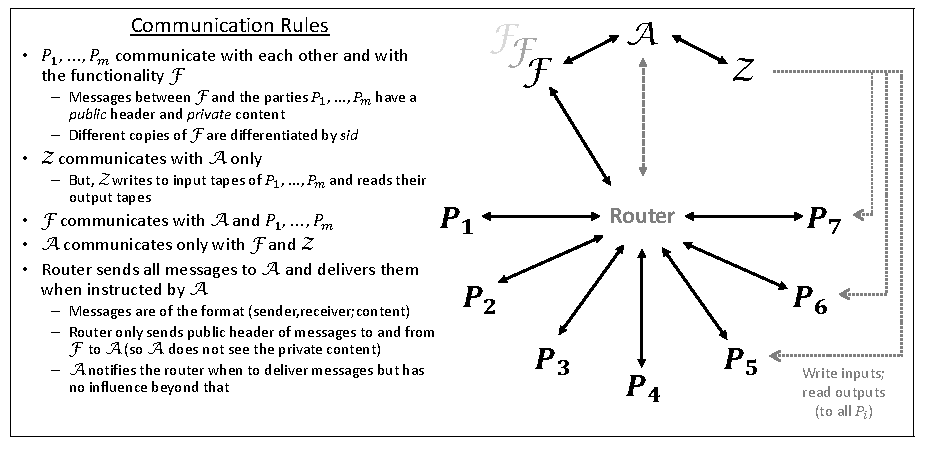
\includegraphics[scale=0.9]{router}
    \caption{The communication model, from the \cite{Canetti_SUC} paper}
    \label{SUC_router}
\end{figure}

The adversary is able to control the router, and thus can delay or block any message. However, the communication is supposed to be authenticated, so the adversary cannot modify its content.

Moreover, any communication between a party and the ideal functionality $\Fun$ is comprised of a \texttt{public header} and a \texttt{private content}; the router forwards to the adversary only the \texttt{public header} part of the message.

Formally, the router operates in the following way:
\begin{itemize}
    \item Read any incoming message of the form $(P_i,P_j,x)$; check that $P_i$ is the actual sender, store it and forward the message to $\adv$.
    \item Do the same for any message from/to the functionality, but only forward to $\adv$ the \texttt{public header}.
    \item When instructed by $\adv$, deliver the message to $P_j$.
\end{itemize}

Notice that in this model of communication we cannot guarantee fairness by definition: all the messages, including the outputs from $\Fun$, may be blocked from the adversary. Moreover, we cannot model local computations (such as encryption) via an ideal functionality, since those calls will be notified to $\adv$ and it might decide to block the output, which is not realistic for a local computation.

Finally, the environment $\zdv$ communicates only with the adversary, and not via the router. However it has access to the input/output tapes of all the parties.

\subsection{Execution and corruptions}

The execution starts from $\zdv$, which is given an input $z\in\bin^\ast$; moreover each machine has the value $\secparam$ in their security parameter tapes.

The environment may at any time write to the input tapes of the parties, read their output tapes or communicate with the adversary.

Then the main loop of execution begins: the adversary reads its incoming communication tape; it can perform any computation and then it may send any of the following messages
\begin{itemize}
    \item Instruct the router to deliver any message; then the receiving party is activated.
    \item Send a direct message to $\Fun$, and activate it.
    \item Send a direct message to $\zdv$, and activate it.
\end{itemize}

Whenever any party is activated, it reads its incoming communication tape, it does whatever computation it needs, and then sends any messages to the router, which will forward all messages to the adversary.

The loop continues until the environment outputs a bit and halts.

Moreover the adversary can corrupt any parties they want, formally by sending a $(\texttt{corrupt}, P_i)$ message through the router. The corrupted party will then follow the adversary instructions, and the environment will be notified.

We will mostly be dealing with \emph{static} corruptions, which means that the adversary can only corrupt a fixed set of parties at the start of the protocol.

There is also the important distinction, as in the stand-alone model, between \emph{semi-honest} and \emph{malicious} adversaries. A semi-honest adversary only gets a read-only access to the internal tapes of a party; this means that the party will follow the prescribed protocol.

In case of a malicious adversary, besides getting access to the internal tapes, the adversary can instruct the router to send any message it wants as the corrupted party, effectively deviating arbitrarily from the protocol.

\subsection{Execution models and security properties}

We are now ready to define real, ideal and hybrid models, from which security definitions and composition theorems will follow. These are special cases of the execution and commuication models described above.

\begin{itemize}
    \item The \emph{real model with protocol $\pi$}: there is no ideal functionality $\Fun$, and all the parties communicate with each other following protocol $\pi$. We denote the output bit of the environment $\zdv$ after an execution of $\pi$ with adversary $\adv$ by $\textsc{\scriptsize SUC-REAL}_{\pi,\adv,\zdv}(n,z)$, where $n$ is the security parameter and $z$ is the input of the environment.
    \item The \emph{ideal model with $\Fun$}: all the parties follow a very simple trusted party protocol. In particular, each party sends to the functionality $\Fun$ precisely the value on their input tape, provided by the environment (unless they are corrupted, thus $\adv$ can make them send anything to $\Fun$). Moreover they write the message returned by $\Fun$ on their output tapes.
    
    We denote the output of $\zdv$ after this ideal execution with $\Fun$ and adversary $\sdv$ by $\textsc{\scriptsize SUC-IDEAL}_{\Fun,\sdv,\zdv}(n,z)$.
    
    \item The \emph{hybrid model with $\pi$ and $\mathcal G$}: the parties follow protocol $\pi$ and communicate with each other, but may be instructed to communicate with the ideal functionality $\mathcal G$. We denote the output of $\zdv$ after an execution of $\pi$ with ideal calls to $\mathcal G$ against adversary $\adv$ by $\textsc{\scriptsize SUC-HYBRID}^{\mathcal G}_{\pi,\adv,\zdv}(n,z)$
\end{itemize}

We finally give our definition of security, which is very similar to the one used in the stand-alone model, but here we have the environment that acts as a distinguisher.

\begin{definition}
    Let $\pi$ be a protocol and $\mathcal F$ be an ideal functionality. We say that $\pi$ \emph{SUC-securely computes} $\mathcal F$ if for any PPT adversary $\adv$ there exists a PPT simulator $\sdv$ such that for any PPT environment $\zdv$ it holds that
    $$ \{ \textsc{\scriptsize SUC-IDEAL}_{\Fun, \sdv, \zdv} \} \cindist \{ \textsc{\scriptsize SUC-REAL}_{\pi, \adv, \zdv} \}$$
    
    If $\pi$ is a hybrid protocol which uses a functionality $\mathcal G$, we instead say that $\pi$ SUC-securely computes $\Fun$ in the $\mathcal G$-hybrid model if
    $$ \{ \textsc{\scriptsize SUC-IDEAL}_{\Fun, \sdv, \zdv} \} \cindist \{ \textsc{\scriptsize SUC-HYBRID}^{\mathcal G}_{\pi, \adv, \zdv} \}$$
\end{definition}

We observe that for any adversary $\adv$ and environment $\zdv$ there exists an environment $\zdv'$ that includes internally the adversary $\adv$ and communicates with a dummy adversary that simply relays messages between $\zdv'$ and the router. Since the definition quantifies over every adversary and environment, for proving SUC-security it is sufficient to emulate this dummy adversary.

Formally, this dummy adversary $\ddv$ receives messages $(i,j,m)$ from the environment and instructs the router to send message $m$ to $P_j$ from the corrupted $P_i$; moreover, it forwards to $\zdv$ any message received from the router. Finally, it forwards any message from/to the functionality $\Fun$ to/from the environment.

We finally can state the following proposition.
\begin{proposition}
    The protocol $\pi$ SUC-securely computes $\Fun$ if there exists a PPT simulator $\sdv$ such that for any PPT environment $\zdv$ we have 
    $$ \{ \textsc{\scriptsize SUC-IDEAL}_{\Fun, \sdv, \zdv} \} \cindist \{ \textsc{\scriptsize SUC-REAL}_{\pi, \ddv, \zdv} \}$$
\end{proposition}

Exactly as in the stand-alone model and in the full UC framework, protocols can be composed while mantaining SUC-security.

Indeed, if $\pi$ is a protocol for computing $\Fun$ in the $\mathcal G$-hybrid model, and $\rho$ is a protocol for computing $\mathcal G$ (eventually in a $\mathcal H$-hybrid model), we can define the protocol $\pi^\rho$ that computes functionality $\Fun$ in the $\mathcal H$-hybrid model. This is done by replacing the code to calls to $\mathcal G$ with the code for executing $\rho$; we only impose the restriction that different instances of $\rho$ call different instances of $\mathcal H$, if $\rho$ is itself hybrid.

We thus have the following composition theorem.
\begin{theorem}
    Let $\pi$ be a protocol in the $\mathcal G$-hybrid model, and $\rho$ a protocol that SUC-securely computes $\mathcal G$ in the $\mathcal H$-hybrid model. Then for any PPT adversary $\adv$ there exists a PPT simulator $\sdv$ such that for all PPT environments $\zdv$
    $$ \{ \textsc{\scriptsize SUC-HYBRID}^{\mathcal H}_{\pi^{\rho}, \sdv, \zdv} \} \cindist \{ \textsc{\scriptsize SUC-HYBRID}^{\mathcal G}_{\pi, \adv, \zdv} \}$$
    
    In particular, if $\rho$ SUC-securely computes $\mathcal G$, then the protocol $\pi^\rho$ SUC-securely computes the functionality $\Fun$.
\end{theorem}

We conclude this chapter with the main motivation for introducing the SUC framework: it's easier to work with with respect to the full UC framework, but it gives the same security guarantees. The only difference is that not all tasks that can be modelled in UC can also be modelled in SUC.

\begin{theorem}
    Let $\pi$ be a protocol that SUC-securely computes the functionality $\Fun$ in the $\mathcal G$-hybrid model. Then there is a transformation $\phi$ such that the protocol $\phi(\pi)$ UC-realizes the functionality $\phi(\Fun)$ in the $(\phi(\mathcal G), \Fun_{\textsc{AUTH}})$-hybrid model.
\end{theorem}

The details of this transformation and the proof of the theorem, along all other proofs of the theorems in this section, can be found in \cite{Canetti_SUC}.